\documentclass{article}
\usepackage{graphicx}
\usepackage{changes}
\usepackage{lipsum}% <- For dummy text
\usepackage{subcaption}
\usepackage{cite}
\usepackage{natbib}
\bibliographystyle{plainnat}
%\bibliographystyle{plos2015}
%\usepackage{plainnat}
%\usepackage[doi=false]{biblatex}
\usepackage{setspace}
\usepackage{tablefootnote}
\usepackage{amsmath}% http://ctan.org/pkg/amsmath
\usepackage{kbordermatrix}% http://www.hss.caltech.edu/~kcb/TeX/kbordermatrix.sty
\usepackage[export]{adjustbox} %http://tex.stackexchange.com/questions/91566/syntax-similar-to-centering-for-right-and-left
\usepackage{authblk} %https://www.overleaf.com/help/75-how-do-i-add-additional-author-names-and-affiliations-to-my-paper#.VZ_wFvlVhBc

\captionsetup{compatibility=false}
\definechangesauthor[name={Per cusse}, color=orange]{per}

%\setremarkmarkup{(#2)}


\newcommand{\beginsupplement}{%
      \setcounter{table}{0}
      \renewcommand{\thetable}{S\arabic{table}}%
      \setcounter{figure}{0}
      \renewcommand{\thefigure}{S\arabic{figure}}%
   }
 
\begin{document}
\title{Inferring influenza epidemic dynamics in the presence of stratified immunity}
\author[1]{Hsiang-Yu Yuan}
\author[2]{Marc Baguelin}
\author[3]{Kin On Kwok}
\author[4]{Nimalan Arinaminpathy}
\author[1]{Steven Riley}
\affil[1]{Medical Research Council Centre for Outbreak Analysis and Modelling, Department of Infectious Disease Epidemiology, School of Public Health, Imperial College London, London, United Kingdom}
\affil[2]{Centre for the Mathematical Modelling of Infectious Diseases, Department of Infectious Disease Epidemiology, London School of Hygiene \& Tropical Medicine, London, United Kingdom}
\affil[3]{School of Public Health, Li Ka Shing Faculty of Medicine, The University of Hong Kong, Hong Kong Special Administrative Region, People's Republic of China}
\maketitle

%\bibliographystyle{style.bst}
%\bibliographystyle{plainnat}
\nocite{*}
% Notes from meeting 11th sept
% - explain precisely the mechanisms wrt boosting and protection and whether they are being inferred or assumed
% - consider a figure about titre and protection 
% - purely biological conceptual model
% - additional intro paragraph
% comparison of model output and sera; boosting and protective effect of titres; dynamics; reproduction number; and sensitivity analysis. Or something that similarly groups the narrative in terms of sero and epi.


\doublespacing
\begin{abstract}
To monitor and control infectious diseases transmission, such as influenza outbreak, it is essential to determine accurately the number of infected cases. However, it is often difficult because the the number of hospitalized cases and the existence of asymptotic infections would lead to a large bias. The serological data provides a good opportunity to estimate disease incidence and to characterize the disease transmission. However, the tool to infer disease dynamics using serological data is required.

Here, we define an epidemic model of influenza in which antibody titre classes are stratified and enumerated explicitly. We fit the model to serological data from the 2009 pandemic in Hong Kong and are able to reproduce key features of the epidemic curve based only on pre- and post-wave serological data. We observe differential antibody boosting with age. Based on our transmission model, we define $R_{B}$ to be the effective reproductive number in the presence of stratified immunity and describe its temporal dynamics relative to the traditional effective reproduction number commonly using 1:40 as the threshold of seroconversion. $R_{B}$ drops rapidly after August and reaches below one in early October. Our results suggest that the disease dynamics and herd immunity of a population can be described more accurately for influenza when the distribution of immunity is explicitly represented, rather than the dichotomy between 'susceptible' and 'immune' states that is often assumed.

\end{abstract}

\section{Introduction}
The basic reproductive number $R_{0}$ allows us to measure the transmission potential of emerging infectious diseases, such as influenza, measles, West Nile virus, dengue,...etc. It is defined as the average number of newly infected cases caused by one typically infected individual in an otherwise naive population (\cite{Heesterbeek2002}). However, analysis based only on the concept of a constant basic reproductive number does not reflect important ecological processes such as changes in behaviour, the impact of interventions nor variability in distribution of immune status of individuals during the course of an outbreak.

The effective reproductive number $R(t)$ is frequently used as an alternative to $R_{0}$ and is defined as the average number of secondary cases per primary case during the course of an epidemic (\cite{Anderson1991}). Values of $R(t)$ are typically calculated in one of two ways: directly from case incidence data under the assumption that $R(t)$ is changing in an arbitrary manner over time (\cite{Wallinga2004},\cite{Wallinga2007},\cite{Grassly2008}); or from a mechanistic model that describes a set of precise ecological assumptions about how the depletion of susceptible individuals or implementation of interventions may be affecting transmission (\cite{Anderson1991}). Although the former method is useful in real-time tracking of the outbreak (\cite{Whoebola2014},\cite{Fraser2009}), to test hypotheses about the underlying drivers of incidence or to predict the impacts of interventions on the incidence, the latter approach is typically used(\cite{Dorigatti2013},\cite{Baguelin2013}). However, only few studies have taken the mechanistic approach as it relies on more understanding of the interplay between immunological and disease dynamics. Recently, a new approach has been developed using a diffusion equation to model the transmission coefficient(\cite{Dureau2013}) and has been used to track the change of transmission during the Ebola outbreak in West Africa(\cite{Camacho2015}). This combines the compartmental modelling approach with more flexibility as the underlying dynamical  process does not have to be described explicitly; however, the immunological protection is simply assumed to be either susceptible or fully protected. 

Serological surveillance for antibodies is often used to identify current and past infections for many infectious diseases. The antibody titres of each individual to influenza infection can be measured using haemagglutinin inhibition (HI) assay (\cite{Hirst1941}). A higher titre is often observed for the individuals who have been infected by the similar virus strain before and is generally correlated to a higher clinical protection, which was observed from a small number of deliberate infection experiments (\cite{Hobson1972} \cite{Dunning2006} \cite{Coudeville2010}). Recently, serological data have been incorporated in a compartmental mathematical model to assess epidemiological mechanisms and to estimate $R(t)$ of influenza outbreaks. For example, Dorigatti \textit{et al.} showed that the increased transmission could explain the third wave of infection, correlated with a higher $R(t)$ determined by both the transmission and waning of the immunity, under the assumption in the model that only individuals with HI titres below a threshold (1:32) are susceptible. Until now, most studies and protocols suggest using a titre of 1:40 (or 1:32 if the sera was diluted from 1:2) as a threshold for seroconversion, as the titre was previously estimated to generate about $50\%$ immune protection (referred to TP50) (\cite{Hobson1972} \cite{Coudeville2010}). Although using a threshold would allow simplicity in mathematical modelling, certain limitations exist while using serosurveillance data to estimate influenza incidence. First, due to a wide variety of antibody boosting observed in serological studies, disease incidence would often be underestimated if low titres are completely ignored (\cite{Wu2014a}). Moreover, TP50 could differ by virus strains and host ages  (\cite{Black2012}). A TP50 higher than the pre-defined threshold could lead to overestimation of the proportion of seropositive (or immune protected) individuals. Another study, which measures a population level mean susceptibility by summarizing individual protection from different titres (\cite{Baguelin2013}), although reflecting the changes of the degrees of herd immunity over time, does not capture the individual varieties of antibody protection or antibody boosting.

Here, we proposed a refinement of the concept of immunity within mechanistic models for influenza. We explicitly enumerated all possible titres in HI assays and mapped them onto a variable scale of susceptibility in different age groups. By coupling a disease transmission model with antibody boosting, we estimated epidemiological and immunological parameters from cross-sectional serological data and described the effective reproductive number during the course of the 2009 influenza pandemic in Hong Kong. By fitting to serological data only during the first peak of pandemic, we reconstructed the disease and serological dynamics and compared them to the classic threshold model.  

\section{Results}
\subsection{Patterns of antibody titres}
We observed both a substantial decrease in the number of individuals with undetectable antibodies and an increase in the proportion of the population with higher HI titres in pandemic influenza serosurveillance data during 2009 in Hong Kong. The pandemic started in early May 2009 with the first confirmed case announced on the 1st of May. Between baseline and the follow-up (Figure S1), the proportion of the study population without detectable antibodies decreased from $89.1\% [86.3\%-91.6\% ]$ to $77.0\% [73.2\%-80.8\%]$ (Figure 1). The amount of increase of detectable titres was distributed more to the individuals with higher titres than T1, for example titres between 1:80 and 1:320 accounted for $65.1\%$ of the decrease observed in the proportion with undetectable titre.

\subsection{Antibody titre distribution}
We constructed a serological-titre model in which each age group and titre class was represented explicitly (see Methods and Figure S2) and estimated the serological responses, clinical protection parameters and initial conditions of the model in a Bayesian framework. Aggregated across age groups, the model was able to reproduce antibody profiles with good accuracy call out. In order to compare the distribution of titres in the data and from the titre model, we examined the titres at the average time of sampling for each round, 11 Aug 2009 (T1) for the baseline recruitment and 22 Dec 2009 (T2) for the follow-up. We first compared the model-predicted distributions of titres to the observed titres for these time points among all age groups in Figure 2. Model titres at T1 were very close to the initial conditions and were slightly lower than certain observed baseline titres but overall were consistent with them. At T2, the proportions of all model predicted titres fell into or overlapped with the $95\%$ confidence interval of the observed follow-up titres. 

Next, we compared the titres for each age group. Children ($\textless20$ yo) had high antibody titres during follow-up while low to medium titres were present in the middle-aged adults (40-64 yo) and elders ($\geq65$ yo) (Figure 2). Although there were some differences in the age specific comparison of model output and observed titres, given the small sample size for some age groups and that pre-existing immunity was not well known, the model fit showed a good agreement with the observed titres. 

The predicted seroprevalence(defined as the proportion of individuals having HI titres $\geq1:40$) from the model output increased from $2.7\%[2.3-3.3\%]$ (T1) to $20.6\%[15.5-24.1\%]$ (T2), which was also in good agreement with the follow-up titres $20.6\%[17.2-24.5\%]$ but slightly lower than the baseline titres $8.9\%[6.6-11.6\%] $(Figure 3A and Table S1. The average increase of seroprevalence was $17.9\%$ which was also consistent but slightly higher than the 16\% [13-18\%] non-age-standardized average rate of seroconversion from a previous study on the same data (\cite{Riley2011}). The largest increase of seroprevalence was shown for children from $2.9\%[2.1-4.2\%]$ to $36\%[26.9-42.5\%]$, and the least change was observed for the elders from $4.1\%[4-4.2\%]$ to $9.9\%[5.4-8.4\%]$, which is consistent to the observed titres and the attack rate $43.4\%$ defined in age group 5-14 yo (\cite{Wu2010}) and other age specific cases reports (\cite{Yang2015}).

To test whether low incidence among elders during the outbreak was mainly caused by higher pre-existing antibody, we also simulated the model in which elders had the same initial antibody protection as other age groups, similar serological patterns were found, which indicates pre-existing antibody in elders would not be the main factors leading to lower incidence this age group.

 
The model-predicted geometric mean titres changed from 2.7[2.5-3.1] (T1) to 4.5[4.1-4.9](T2), consistent to the increase of the geometric mean titres of the observed sera from 3.8[2.3-5.3] to 4.8[3.5-6.1] (Table S2). The predicted geometric mean titres at T2 were highest among children and decreased by age, which agreed with observed sera.

\subsection{Reproducing epidemic dynamics}
Fitting only serological data, the titre model was able to reproduce key features of the incidence of influenza infection in Hong Kong during the initial wave of the 2009 pandemic. The average incidence increased rapidly after August and reached the peak in early October (Figure4A). In the model, the incidence peak occurred on 10 Oct 2009 [2 Oct - 18 Oct], which was close to the peak incidence of hospitalization of confirmed cases in fourth week of September on the assumption of 2-3 weeks delay of the development of the boosted HI titres  (\cite{Wu2010} \cite{Riley2011} figure S1). The model estimated a cumulative incidence between baseline and follow-up of $21.4\% [15.5\% - 26.0\%]$ which is  higher than the total average increase of seroprevalence for the study population because low antibody boosting and reinfection from partial protection were neglected using seroprevalence. The model reproduced a longer tail in the epidemic profile after November until the disease faded out.

The rapid increase in population titres at the end of August can be seen in the timeseries of population immunity described by the titre model result (Figure 4B). The constant red bands up to August reflected our assumption that pre-existing antibodies in each age group were uniform between 1:10 and 1:80 and that incidence did not reach a substantial proportion of the population until the end of the summer. Once incidence did increase, a large proportion of individuals showing titres between 1:40-1:320 after seroconversion. The pattern of antibody response was approximately constant after January once the titre model incidence faded out.

Our model results were different from those obtained from a traditional threshold SIR model. To compare the results to the traditional method using 1:40 as seroconversion threshold, a similar analysis was performed using the threshold model (same as the classic SIR model) with the same age mixing effect. A slightly lower cumulative incidence was estimated from T1 to T2, 16.9\% [12.3-22.4], the date of incidence peak was estimated to be 7 Nov 2009[20 Sep - 1 Dec], which is nearly one month delayed than the titre model (Figure 4C). Rapid seroconversion occurred during late October and November corresponding a higher incidence during those periods(Figure 4D). The increase of seroprevalence in the threshold model was showing less agreement with the observed titres (Figure 3B) than the titre model predicted output. 
 
\subsection{Effective reproductive number}
To measure the transmissibility during the influenza pandemics in a heterogeneous population, we calculated the effective reproductive number $R_{B}$ in the presence of pre-existing antibodies under the titre model. $R_{B}$ declined slowly from 1.22[1.16-1.28] in the first four months of the outbreak, dropped rapidly below one during September and October, and became stable at 0.82[0.78-0.92] after November while disease were fading out (Figure 5). The mean $R_{B}$ was calculated and reached 1 on 6 Oct, near the time when disease incidence reached the peak and started to decay. The distribution of the time when $R_{B}$ equals 1 was same as the peak time of incidence. However, because we plotted the credible interval $R_{B}$ by time in Figure 5, the interval of the time when $R_{B}$ fell to 1 became larger than the credible interval of the incidence peak.

Using the threshold model with the same age mixing effect and same proportion of pre-existing immunity, the range of the effective reproductive number (denoted as $R_{C}$), decreasing from 1.19 [1.16-1.25] to 0.82 [0.79-0.86] during the time of outbreak, was similar to $R_{B}$. However, the main difference between $R_{B}$ and $R_{C}$ was the timing of the reproductive numbers falling below 1. The mean $R_{C}$ dropped to one on 11 Nov 2009, which was 1 month later than $R_{B}$, corresponding to the delay observed from both of the disease incidence and seroconversion (Figure S4).


\subsection{Age-specific boosting}
We estimated significant differences in age specific antibody boosting following the infection. The mean antibody boosting was highest among children (5.96 [4.98-0.057]), with near 64-fold increase in titres. The boosting decreased by age until middle-aged adults to near 16-fold increase (3.78[3.03-4.60]), whereas elders showed a higher boosting than middle-aged adults (Table 1).

We did not find significant evidence for age-specific correlates of immune protection. The protective titres which associated with 50$\%$ protection (TP50) were not significantly different by ages. Among the children and adults, the average protective titres were between 1:20-1:80, which was consistent to several previous studies (\cite{Hobson1972} \cite{Coudeville2010}). For young adults, given the protective titre near 1:80 and the differential susceptibility (defined as eq5), a large number of individuals with detectable antibody showed titres $\leq$ 1:40 during the baseline round can only be partially protected. However, for middle-aged adults, the average protective titres were between 1:20-1:40, which suggested that the low induced boosting may be offset by a higher level of protection (Table 1). For elders, a weaker protective titre is found between (1:160-1:320) but with a wider credible interval. 


\subsection{Sensitivity analysis}
To determine the effect of the initial infecteds $T_{0}$ on the disease dynamics, we estimated the disease dynamics using different numbers of initial infecteds seeding the population on 1st May. When the initial infecteds was reduced to one, the peak were largely delayed to December in both titres and threshold models (Figure S6). Nonetheless, due to the stochastic effects for disease to start spreading, extreme lower infecteds number would often lead to lineage extinction without creating a disease pandemic. Therefore, a higher number of $T_{0}$ could be often the case to lead a major outbreak. For example, to prevent disease stochastically fade out during the early stage given $R_{0}=1.25$, the initial infecteds $T_{0}$ would need to be larger than 10 such that the probability of a major outbreak $1-{(\frac{1}{R_{0}})}^{T_{0}}$ is not less than $90\%$ (\cite{Allen2012} \cite{Hartfield2013}). When $T_{0}$ was increased from 10 to 100 individuals, the incidence peak occurred slightly earlier from the early of the October toward the late September in the titre model. In contrast, the peak dropped largely from mid November to late September in the threshold model. Given the intensive surveillance were conducted in Hong Kong and also globally before May 2009 (\cite{Fielding2010}) and increased pathogenicity in the pandemic strain, it is unlikely the initial infecteds could become greatly larger than one. In this study we set 10 initial infecteds at the beginning of the outbreak. 


\section{Discussion}
We have developed a serological model for the transmission of influenza in which individual antibody titre levels are enumerated explicitly. The model provides a framework to estimate the disease dynamics using time series cross-sectional serosurveillance data, which is easier to perform than longitudinal study. This model structure allows us to define the effective reproduction number $R_{B}(t)$ by time as the transmissibility of an influenza strain in a population that contains pre-existing and changes of immunity, as reflected by antibody titres. By estimating the parameters of the model using cross-sectional serological data from the 2009 pandemic in Hong Kong, we are able to explain age-specific patterns of antibody boosting, protection and overall cumulative incidence. A significant higher antibody boosting was observed for children. However, both titres and threshold models could predict a larger increase in seroprevalence for children and little increase in elders. The reason why less incidence occurred among elders could not be explained by the difference of pre-existing antibody, and was probably caused by the contact mixing and the age-specific relative virulence.   
  
Our analysis suggests that the 2009 pandemic strain have an underlying $R_{B}(0)$ of ~1.22 in the presence of the pre-existing or cross-reactive antibodies, which is slightly lower or consistent other studies using laboratory confirmed illness in Hong Kong (\cite{Cowling2010}, \cite{Wu2010}, \cite{Wu2014} \cite{Grund2011}). The time of $R_{B}$ dropping below one is slightly later with the incidence peak of the Hong Kong pandemic using hospitalized cases (\cite{Riley2011}). However, the delay could happen considering serological response occur few days upto 3 weeks later infection (\cite{Mak2010}, \cite{Miller2010}). Comparing to the traditional threshold SIR model, the $R_{B}$ is better supported by the incidence peak. The main difference of disease dynamic between $R_{B}$ and $R_{C}$ is the huge delay of the incidence peak in the threshold model, which could be explained by the following. The threshold SIR model underestimated the incidence number in early baseline period due to there are nearly $20\%$ of individuals having titres $\textless 1:40$, which  would be ignored as seronegative. However, during follow-up round, the main increase happened for the individuals showing titres higher than $1:40$. Together, this resulted in an underestimate of infection during baseline period which produced a bias of the seroconversion toward the late pandemic period when $1:40$ threshold titre is used. 
  
The finer immune structure improves the disease dynamics prediction not only because low antibody boosting could be considered but also the partial protection for different titres could be estimated. With partial protection, individuals with weak to medium pre-existing immunity could still be infected. The longer tail of disease incidence observed in influenza pandemic in Hong Kong after December reflects this partial protection. Among our sera data, 14.5$\%$ of infected individuals were seroconverted from pre-existing positive antibody titres (data not shown), indicating a higher possibility of secondary infection or tertiary infection in the population. The occurrence of the re-infection could explain why an increase of the proportion of higher titres exists during follow-up round. In general, multiple infections of the same individuals can occur when no or only partial immune response are elicited after infection as a result of antigenic drift or waning of immunity (\cite{Heesterbeek2015}). However, our study highlights how multiple infections may occur even within the span of a single epidemic, once a spectrum of immune protection is permitted in the model, the peak and the tail of the disease incidence could be estimated much closer to observed incidence patterns, leading a better prediction of disease dynamics than the threshold model.


One of the most important challenge for infectious disease control is to real time monitor disease transmissibility by estimating effective reproduction number $R(t)$ (\cite{Cowling2010}). Serological titre model provides a different approach for monitoring disease transmissibility other than counting actual cases reports. The concept of this approach can be applied on serological studies on other infectious diseases, such as severe acute respiratory (SARS), Middle Eastern respiratory syndrome (MERS), HCV, West Nile virus,...etc. Once early estimates of antibody boosting and protective titres are obtained, this method can infer the effective reproductive number and the disease dynamics , which are valuable for infectious disease monitoring, controlling and prediction.

\section{Materials and Methods}

\subsection{Serological samples}
We analyzed new data from the baseline and the follow-up rounds of the Hong Kong influenza serological survey \cite{Riley2011}. Here, we used haemagglutination inhibition assay results for the 2009 pandemic strain of H1N1. We obtained the baseline HI titres from 523 individuals (between 4 Jul 2009 and 28 Sep 2009), and from 465 individuals recruited during the follow-up (between 11 Nov 2009 and 6 Feb 2010) (Figure S1). Previously published analyses used microneutralization assay results only for the subset of individuals with paired samples. We also noted that previous analyses was based only on fourfold rise or greater in paired samples and thus did not need to exclude individuals who reported vaccination prior to the baseline visit. Here, because it was our objective to make inference on cross-sectional patterns of serology, for our primary analyses, we excluded all individuals who reported any influenza vaccination in the preceding years.

\subsection{Transmission Model}
The epidemiological and serological dynamics were simulated based on a disease transmission model with a serological response component. The serological model without age mixing effects is illustrated in the Figure S2 by the extension of the susceptible infected recovered susceptible (SIRS) model to multiple levels, where each level represented a different antibody titre. Once an individual became infected, viruses could transmit to other susceptible individuals during the infectious periods. The transmission susceptibility for the titre given a contact was obtained based on the differential susceptibility. A higher antibody level would reduce the susceptibility of individuals(Figure S3A). Once the individual got infected, the antibody was boosted to a higher level according to a truncated Poisson distribution (Figure S3B), which generally captured the antibody titres profiles as seen in the Figure 1. After recovery, the infected individual became temporarily fully protected by both Cytotoxic T lymphocytes (CTL) mediated within 25 days. At the same time, the antibody titres would be boosted to an elevated level. The individuals later became re-susceptible again after the CTL immunity waned and were protected by only antibody titres.

Disease dynamics are described by the following equations while age mixing effects are considered. The model has not taken into account the demographics since the duration of the outbreak we considered here was less than one year. The birth and death rates would not produced significant different outcomes.

\begin{equation}
 \label{simple_equation}
 %\alpha = \sqrt{ \beta }
 \frac{dS{i}(a)}{dt}=-S_{i}\cdot\rho(i)\cdot\lambda(a)+\omega\cdot R_{i}(a)
\end{equation}

\begin{equation}
%\begin{split}%
 \frac{dI{i}(a)}{dt}=S_{i}\cdot\rho(i)\cdot\lambda(a)+\frac{1}{T_{g}}\sum_{j=i}^{i_{max}} I_{i}(a)\cdot g_{ij}
%\end{split}%
\end{equation}

\begin{equation}
 \frac{dR{i}(a)}{dt}=\frac{1}{T_{g}} \sum_{j=i}^{i_{max}} I_{i}(a)\cdot g_{ij}
\end{equation}

where $a$ represents the age group for each individual, $\rho(i)$ is the disease susceptibility for susceptible individuals in the presence of titres level , $\lambda$ is force of infection, $\omega$ is waning rate for CTL immunity. $T_{g}$ is the duration of infection, $g_{ij}$ is the probability of immune boosting from titres $i$ to $j$. The force of infection on member of age class $a$ who are completely naive within the population is 
\begin{equation}
 \lambda(a)=\beta\sum_{b=1}^{a_{max}}{\Big\{m_{ab}\sum_{i=0}^{i_{max}}f_{b}\cdot I_{i}(b)\Big\}}
\end{equation}

where $\beta$ is the basic unit of transmission rate, $m_{ab}$ is the contact rate from the age class $b$ to $a$, $f_{b}$ is the relative virulence of viruses. We stratified sera samples into age groups, i.e. children and adolescent (2-19 y/o; for convenience, we defined this group as children throughout the study), young adults (20-39 y/o), mid-age adults (40-64 y/o) and elders ($\geq$= 65 y/o). Contact mixing matrix of the four age groups was calculated from a community study in Hongkong (Figure S4).

\subsection{Differential susceptibility}
The susceptibility $\rho$ is defined as $1-\phi$ where $\phi$ is the proportion of individuals that are protected from infection given a titre level. The protection is modelled in a two parameters logistic function.

\begin{equation}
 \phi(i) = \frac{1}{1+e^{I_{\beta}({i}-I_{\alpha})}}
\end{equation}
where $I_{\alpha}$ is defined as the antibody titre TP50, which is the titre, at which $\phi$ will drop $50\%$ from the maximum value (Figure S3A). $I_{\alpha}$ will be present as $\mathit{TP50}$ in our study. $I_{\beta}$ determines the shape of the curve.

\subsection{Parameters estimation}
The posterior distributions of the parameters, including the transmission rate $\beta$, 4 age dependent antibody boosting $AbB_{a}$, 4 parameters for immune protection $\mathit{TP50_{a}}$, and 1 for relative virulence of children $f_{1}$, were obtained from Metropolis-Hastings in Markov Chain Monte Carlo with 2x$10^{6}$ steps (Table1) to guarantee each ESS is higher 100. Three parameters of initial conditions were the number of the initial infected individuals, initial pre-existing titres and the relative virulence for children.
   
The prior for all the parameters were set uniform distributed except the variable for $f_{1}$. The starting day of pandemic was set on 1st May (the date of the first observed case in Honk Kong pandemic). We assumed the number of the initial infected individuals was 10, that seeded to the population to cause a major outbreak with only near $10\%$ going stochastic extinction when $R_{0}$ equals 1.25. The seroprevalence was lower than $3.3\%$ prepandemic seroprevalence data using MN assay in Hong Kong(\cite{Wu2014}) because it was shown that MN assay titres were generally more sensitive than HI assay  (\cite{Grund2011}), the initial baseline antibodies among 1:40-80 and 1:10-20 were set to be $2\%$ for age groups $<65$ and was $4\%$ among the same titres groups to represent a higher seroprevalence in elders. The mean relative virulence is set to be 4 with standard deviation equals 1. Likelihood is calculated as
\begin{equation}
  L(\theta|e_{t1},e_{t2},...,e_{tn})=\prod_{i=1}^{n} f(e_{ti})
\end{equation}
where n is the total number of the samples and $f(e_{ti})$ is the frequency of the titres $e$ at time $t$ for the individual $i$.

\clearpage
\subsection{Calculating effective reproductive number}
The effective reproductive number was calculated using next generation approaches. Following the same notations in the study by \cite{Diekmann2010}, the transmissions matrix $T$ and the transitions $\sum$ can be obtained. Each element in $T$ represents the newly 'transmitted' cases in age group $a$ and titres $i$ in a unit time per each infected individual in age group $b$ and titres $l$, which can be calculated as   $  \frac{\lambda(a) \cdot S_{i}(a)}{I_{l}(b)} = \beta h_{i}(a) f_{a} M_{ab}S_{i}(a)$. $\sum$ represents the transitions of between cases in each age and titres group. Since the probability of boosting to all the other titres becomes one, each element in $\sum$ simply is the loss of infected cases due to recovery in a unit time $-\frac{1}{T_{g}}$ from our model.



\pagebreak
\section{Acknowledgement}
We thank Dr. Edwin VanLeeuwen for his valuable comments. The study was supported by xxx Grantxx.
\section{Figures}
\begin{figure}[h!] %h! makes section title above the Figures
      \centering
      %\begin{subfigure}[t]{0.3\textwidth}
      %http://tex.stackexchange.com/questions/17734/cannot-determine-size-of-graphic
              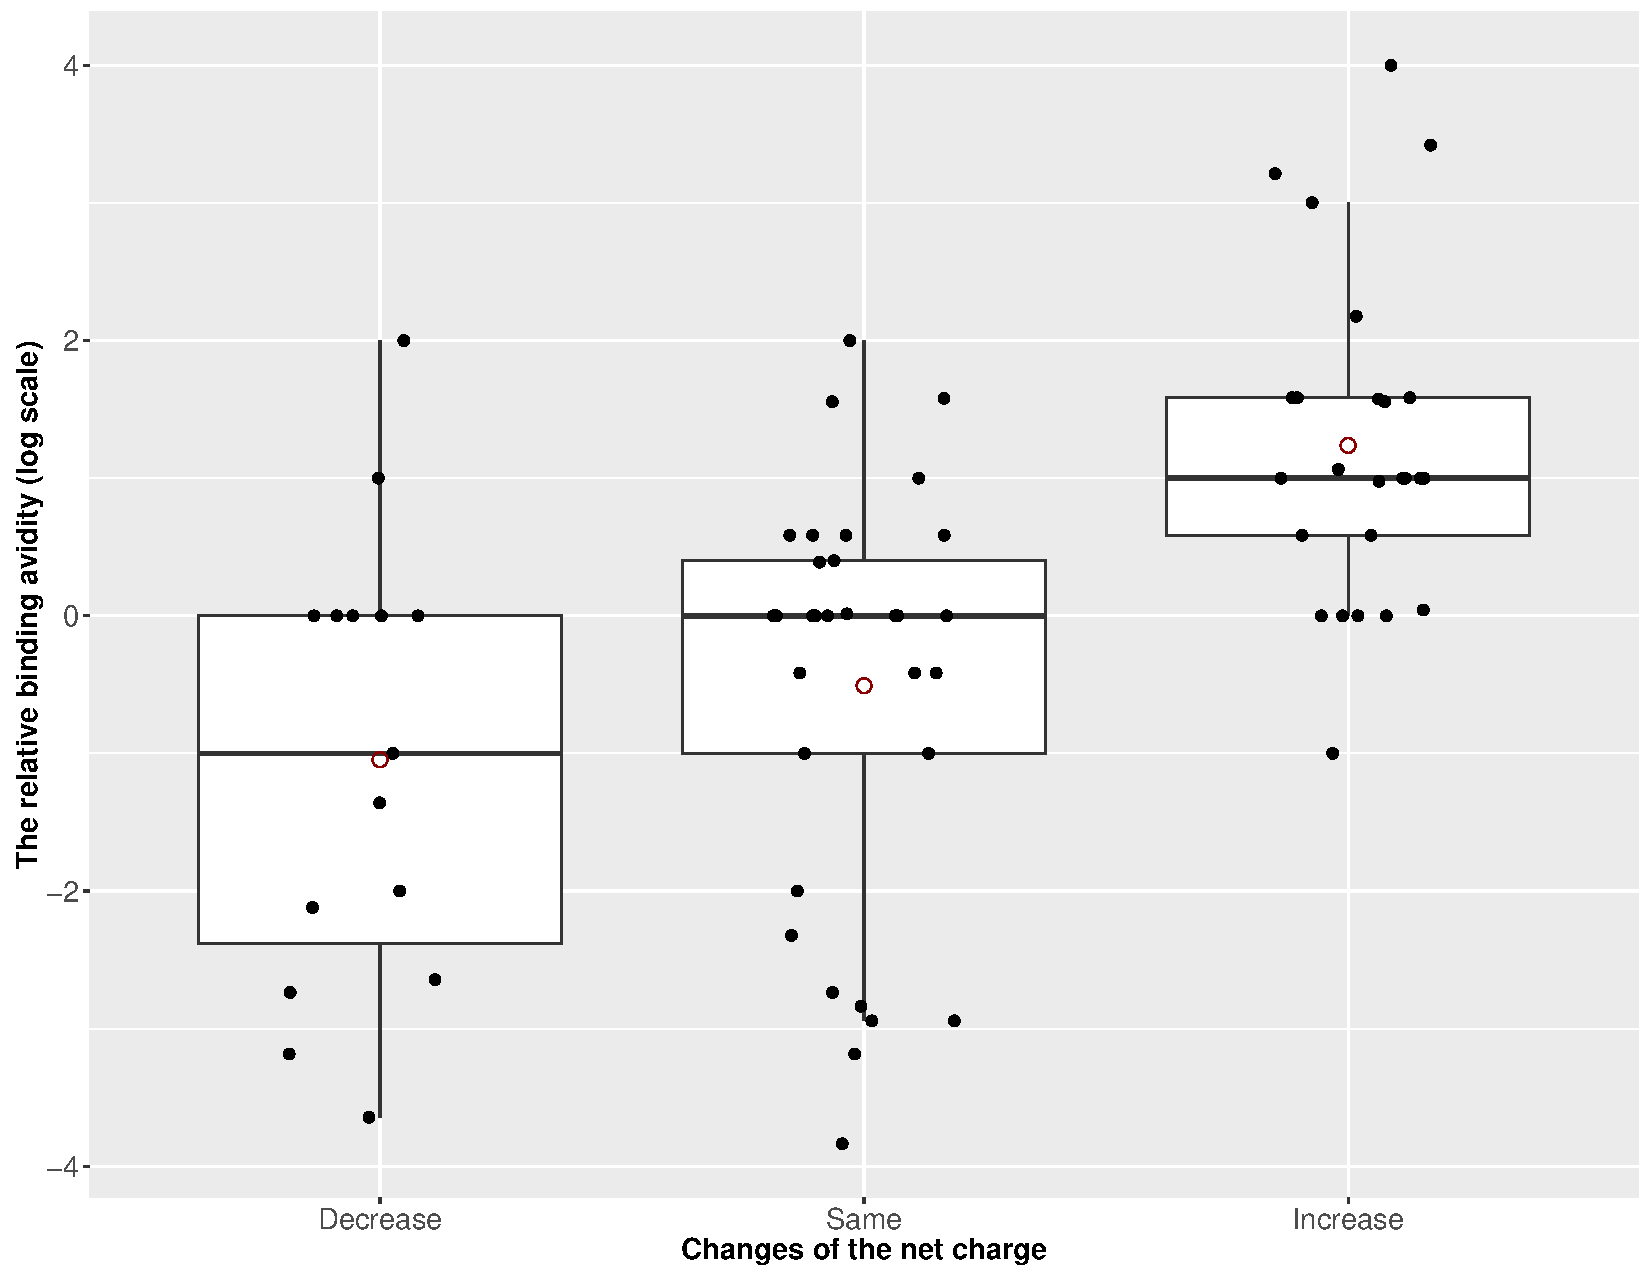
\includegraphics[width=1\textwidth,natwidth=10,natheight=10]{fig/figure1.png}
              %\includegraphics[width=0.8\textwidth,natwidth=610,natheight=642]{tiger.pdf}
              \caption{The serological profiles of naive (left y-axis)and immune population (right y-axis) during the baseline and the follow-up rounds. Dark blue bars represent the baseline titres whereas light blue bars represent followup titres. Left y-axis indicates proportion with undetectable titre. Right Axis indicates proportions in other titre classes. Note left and right y-axis are different scale.}
      %\end{subfigure}
\end{figure}
\clearpage

\begin{figure}[h!]
      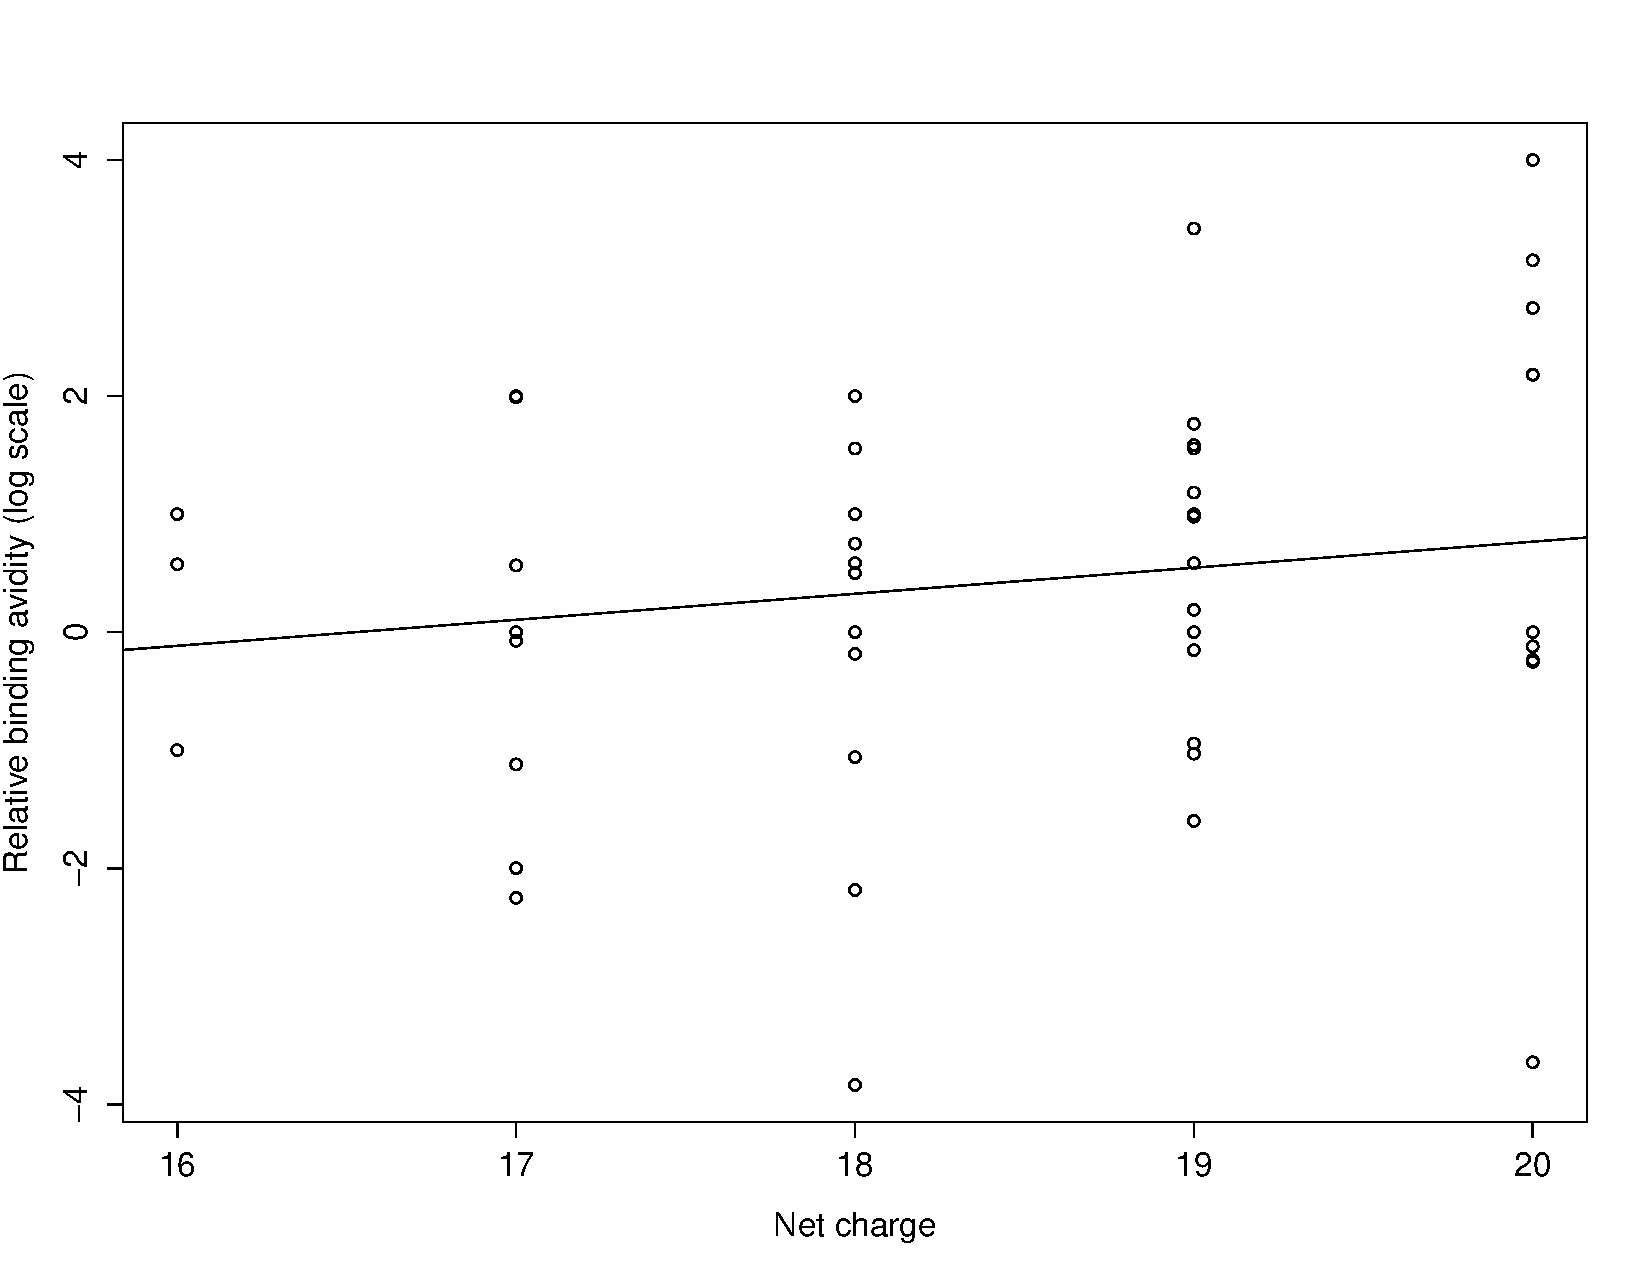
\includegraphics[width=1.2\textwidth,natwidth=8,natheight=8]{fig/figure2.png}
      \caption{Simulated and the observed sera at baseline and follow-up. Top row describes pattern for the entire population. Bottom four rows describe patterns for age groups. Vertical bars indicate $95\%$ binomial confidence intervals (observed) and $95\%$ region of posterior credibility (model). Left and right y-axis as per Figure 1. Blue bars represent the observed titres where gray bars represents the model titres.}
\end{figure}

\begin{figure}[h!]
      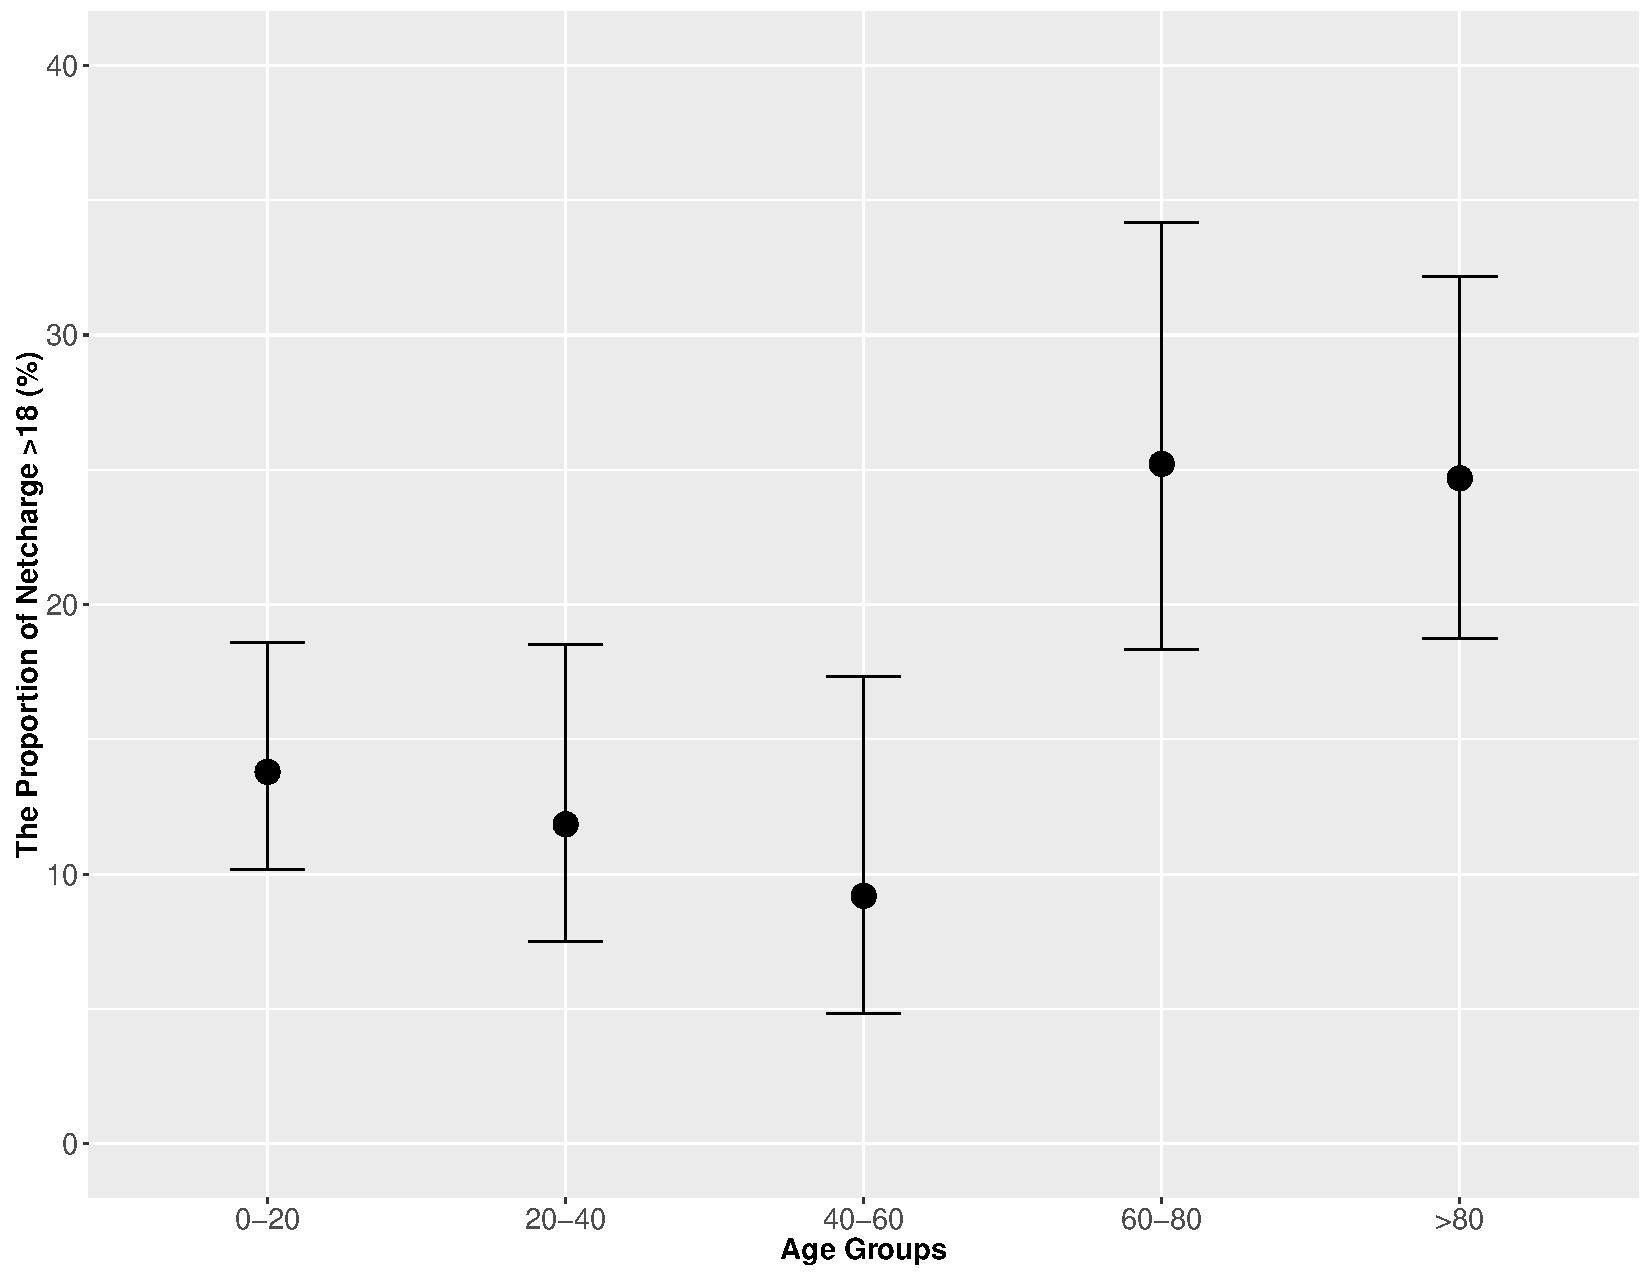
\includegraphics[width=1\textwidth,natwidth=12,natheight=12,height=5.2cm]{fig/figure3.png}
      \caption{The seroprevalence (percentage of individuals with titres  $\geq 1:40 $) from the observed sera and the model output during baseline and follow-up periods among different age groups. (A) The predicted seroprevalence from the titre model. Darker blue represents the observed sera at baseline where lighter blue represents the observed sera at the follow-up; Darker gray represents the simulated sera at baseline where lighter gray represents the simulated sera at the follow-up. (B) The predicted seroprevalence from the threshold model. The colours are same as in (A)}
\end{figure}

\clearpage
\begin{figure}[h!]
      \includegraphics[width=1.102\textwidth,natwidth=8,natheight=10]{fig/figure4.png}
      \caption{The disease and the serological dynamics of the model simulation. The dynamics were reconstructed using 400 random samples from posterior distributions (A) The disease dynamics calculated using the titre model. Blue, susceptible individuals are defined as individuals who show titres less than 1:40. Bolded blue, immune protected individuals are individuals showing titres $\geq1:40$. Solid lines represent the mean of simulation results from posterior distribution. Dashed lines represent $95\%$ credible intervals. Infected are plotted in red (B) The sera dynamics are simulated during the outbreak using the titre model. Darker colour represents a lower proportion and lighter represents a higher proportion in the population. (C) The disease dynamics calculated using the threshold model with the classic definition of seropositive (1:40). Colours are same as in (A). (D) The serological dynamics are simulated during the outbreak using the threshold model. Seronegative ($\textless 1:40$) represents susceptible while seropositive ($\geq1:40$) represents recovered individuals. The darker colour represents a lower proportion and the lighter one represents a higher density in the population.
}
\end{figure}

\begin{figure}[h!]
      \includegraphics[width=1\textwidth,natwidth=10,natheight=10,height=8cm]{fig/figure5.png}
      \caption{The comparison of the effective reproductive numbers between the titre model and the threshold model. Blue, the $95\%$ credible interval of the reproductive number $R_{B}$ estimated from the titre model with age-specific serological parameters. Red, the $95\%$ credible interval of the reproductive number $R_{C}$ estimated from the threshold model with the same age mixing effect. Bolded lines represent the mean values.}
\end{figure}

\clearpage
% Table generated by Excel2LaTeX from sheet 'Table1'
\begin{table}[ht]
\begin{minipage}{\textwidth}      
% Table generated by Excel2LaTeX from sheet 'Table1'
\centering % used for centering table
\caption{The parameters estimation from the titre model and the threshold model using MCMC. The miminum ESS is above 100.}
% title of Table
\centering % used for centering table
\begin{tabular}{rrrr}

\hline\hline \\%inserts double horizontal lines
Parameters* &          Titre Model &        Threshold Model\\ \\
\hline %inserts double horizontal lines
   
    $R_{0}$ &	      1.22 [1.16-1.28] &	1.19 [1.16-1.25]  \\ \\
  
    $AbB_{1}$ &     5.96 [4.98-7.00] &    	- \\ \\

    $AbB_{2}$ &     4.97 [4.02-6.02] &    	- \\ \\

    $AbB_{3}$ &     3.78 [3.03-4.60] &    	- \\ \\

    $AbB_{4}$ &     4.79 [2.16-7.54] &    	- \\ \\
  
    $\mathit{TP50_{1}}$ &    2.15 [0.61-5.41] &  		- \\ \\

    $\mathit{TP50_{2}}$ &    3.40 [0.67-9.13] &  		- \\ \\

	$\mathit{TP50_{3}}$ &    2.80 [0.60-9.05] &  		- \\ \\

    $\mathit{TP50_{4}}$ &    5.76 [0.77-9.69] &  		- \\ \\

    $f_{1}$*          &   	5.01 [3.96-5.95]&         4.57 [3.63-5.58] \\ \\ 
\hline
\end{tabular}
\end{minipage}
\end{table}
Note that $R_{0}$ is defined in the presence of the initial partial immunity here.
\\
*We used uniform priors for all parameters other than $f_{1}$. For $f_{1}$, we used Gaussian distribution with mean=4 and standard deviation=0.5. See figure S5.
\newpage

%\bibliographystyle{unrst}
\bibliography{mymend}
\newpage
\section{Supplementary}
\beginsupplement
\subsection{Serosurveillance}
\begin{figure}[h!]
      \includegraphics[width=0.8\textwidth,natwidth=8,natheight=10]{fig/supp/figureS1.png}
      \caption{Weekly sampling distribution of baseline and follow-up recruitments during pandemic H1N1 in Hong Kong. We obtained the baseline HI titres from 523 individuals (between 4 Jul 2009 and 28 Sep 2009), and from 465 individuals recruited during the follow-up (between 11 Nov 2009 and 6 Feb 2010) during early and post pandemic. The laboratory confirmed cases in Hong Kong are plotted for each week (\cite{Riley2011}). The peak of the incidence occurred in the end of September.}
\end{figure}
  \clearpage

\subsection{Transmission model}
\begin{figure}[h!]
      \includegraphics[width=0.8\textwidth,natwidth=8,natheight=10]{fig/supp/figureS2.png}
      \caption{The illustrated schema of serological model without age mixing effects. In our simulation, the average infectious period $T_{g}$ was 3.3 days. We assumed the recovered individuals \textit{$R$} are temporarily fully protected by T cell immunity which would last 25 days on average (\cite{Kaech2012}). After immunity wanes, recovered individuals become re-susceptible again which are protected by antibody titres only. The susceptibility is defined by two parameters logistic equation in eq5. The shape parameter $I_{\beta}$ was assumed to be 2.102 according to a previous study (\cite{Coudeville2010}). Individuals with a lower titre are more susceptible by infection. Each time after recovery, the titres will be boosted to a higher titres. We assumed the maximum measurable titres $k$ is 1:2560. Any titres larger than this value would be treated as 1:2560 in our model. The total population size is assumed to be $7\cdot10^{6}$.}
\end{figure}

\clearpage

\begin{figure}[h!]
      \includegraphics[width=0.8\textwidth,natwidth=8,natheight=10]{fig/supp/figureS3.png}
      \caption{The differential susceptibility and antibody boosting. A. Susceptibility of individual having different titres. 3 $\mathit{TP50}$, 1:20, 1:40, and 1:160 were used to show susceptibility from higher to lower protection. B. The probability distribution of antibody boosting after the infection.}
\end{figure}
\clearpage


%\begin{figure}[h!]
      %\includegraphics[width=1\textwidth,natwidth=10,natheight=6]{figureS2a.png}
      %\caption{serological profiles of naïve and immune population at sample collecting time  T1 and T2}

%        \includegraphics[width=1\textwidth,natwidth=10,natheight=6]{figureS2b.png}
%        \caption{Attack rate among different age groups. a, calculated from the model. %b, calculated from the sera samples. Red represents the individuals with prexisting %antibody before being infection. Blue represents the individuals are naive before %being infection.}
%\end{figure}

%\begin{figure}[h!]
      %\includegraphics[width=1.4\textwidth,natwidth=10,natheight=10]{figureS3.png}
      %\caption{The distribution of antibody boosting using paired sera from initial %to the follow-up rounds}
%\end{figure}

\begin{figure}[h!]
      \includegraphics[width=1.0\textwidth,natwidth=10,natheight=10]{fig/supp/figureS4.png}
      \caption{ Average daily number of contacts made between age classes between age classes. Bluer colours indicate mixing between age groups less than 1 individual, and yellower colours indicate mixing more than 1 individual. 95\% confidence intervals are shown in the parenthesis, derived from 1,000 re-samples of participant contact diaries. Noted that those one diary from randomly drawn from participants who provided more than one diary in each run of bootstrap. To quantify and describe the tendency of people to mix with others of similar ages or different ages, age contact matrix of participants were constructed based on four waves/rounds of recruitment of the longitudinal telephone contact survey (\cite{KwokInprep}) with four groups of age of participant as columns (2-19,20-39,40-64,65+) and five groups of age of contacts (0-19,20-39,40-64,65+) as rows were calculated based on the number of daily contacts between individuals made based on their age groups.}
\end{figure}

\clearpage

\begin{figure}[h!]
      \includegraphics[width=1.2\textwidth,natwidth=8,natheight=10]{fig/supp/figureS5.png}
      \caption{Posterior distributions of the parameters in the serological titre model. We use uniform priors for all parameters other than $f_{1}$. For $f_{1}$, we use Gaussian distribution with mean=4 and standard deviation=0.5 because of 4 folds increase of viral loads was observed for children for pH1N1(\cite{Lee2011}). The Gaussian prior is plotted in red line. All 4 $TP50$ parameters show little correlation where the maximum correlation coefficients is 0.19 occur between $TP50_{1}$ and $TP50_{3}$.}
\end{figure}

\subsection{Sensitivity Analysis}
\begin{figure}[h!]
      \includegraphics[width=1.2\textwidth,natwidth=8,natheight=10]{fig/supp/figureS6.png}
      \caption{The mean time of incidence peak among different number of the initial infecteds T0. Blue is the estimate of the titre model. Red is the estimate of the threshold model.}
\end{figure}

\clearpage

\begin{table}[ht]
\begin{minipage}{\textwidth}   
% Table generated by Excel2LaTeX from sheet 'Table2a'
% Table generated by Excel2LaTeX from sheet 'Table1'
\caption{The comparison of the seroprevalence observed sera and the titre model output. The seropravalene (\%) among each age group during the baseline and the follow-up rounds are listed. } % title of Table
\centering % used for centering table
\begin{tabular*}{13cm}{rrrrrrrrr}

\hline\hline \\%inserts double horizontal lines

  &  \multicolumn{2}{c}{Observed}  & &  \multicolumn{2}{c}{Model output} \\
 \cline{2-3}  \cline{5-6} \\
 Ages &  Baseline &       Follow-up &   &     Baseline &      Follow-up   \\
\hline \\ %inserts double horizontal lines
 All &     8.9 [6.7 11.6] &    20.6 [17.2  24.5] & &   2.7 [2.3 3.3] &    20.6 [15.5  24.1] \\ \\
 $\textless $20  & 17.7 [10.4 29.5] & 45.5 [33.7 59.4] & & 2.9 [2.1 4.2] & 36 [26.9  42.5] \\ \\

 20-39 &     10.5 [6.0  18.0] &   23.2 [16.2 32.8] & &     2.4 [2.1 3] &   19.9 [14.9 23.4] \\ \\

 40-64 &     5.1    [3.2   8.2] &    9.4 [6.5  13.5] & &   2.4 [2.1 2.9] &    18.7 [13.4 22.6] \\ \\

 $\geq65$ &   4.8  [1.5 16.2] &    15.0 [7.3  29.8] & &    4.1 [4 4.2] &  9.9 [5.4 8.4] \\ \\
\hline %inserts double horizontal lines
\end{tabular*}
\end{minipage}
\end{table}

\clearpage

\begin{table}[ht]
\begin{minipage}{\textwidth}   
% Table generated by Excel2LaTeX from sheet 'Table2a'
% Table generated by Excel2LaTeX from sheet 'Table1'
\caption{The geometric mean titres (the log scale of the titration) of baseline and the follow-up rounds from the observed sera and the model output.} % title of Table
\centering % used for centering table
\begin{tabular*}{13cm}{rrrrrrrrr}

\hline\hline \\%inserts double horizontal lines
&  \multicolumn{2}{c}{Observed}  & &  \multicolumn{2}{c}{Model output} \\
 \cline{2-3}  \cline{5-6} \\
 Ages &  Baseline &       Follow-up &   &     Baseline &      Follow-up   \\
\hline \\ %inserts a horizontal line
  All 				&  3.8 $\pm1.5$ &   4.8 $\pm1.3$ & &   2.7 [2.5  3.1] &   4.5 [4.1 4.9] \\ \\

  $\textless $20  	&  3.9 $\pm1.4$ &   5.8 $\pm1.8$ & &   3.1 [2.6  3.8] &   5.6 [4.8 6.3] \\ \\

  20-39 			&  4.1 $\pm1.6$ &   4.9 $\pm1.5$ & &   2.7 [2.5  3] &     4.7 [3.9 5.5] \\ \\

  40-64				&  3.5 $\pm1.7$ &   3.7 $\pm1.7$ & &   2.6 [2.5  2.9] &   3.8 [3.2 4.5] \\ \\

  $\geq65$ 			&  2.7 $\pm0.5$ &   3.6 $\pm1.5$ & &   2.5 [2.5  2.6] &   3.3 [3.3 4.1] \\ \\
\hline %inserts a horizontal line
\end{tabular*}
\end{minipage}
\end{table}


            
\end{document}


